\chapter{Introduction}
\label{chap:Introdu}
In modern systems distributional models are dominant for a semantic parser. We use graph based methods and apply it to the \textit{2018 Semeval task on Machine Comprehension} (MC). We built a REST-API (available at \url{http://hlt.bme.hu/4lang}) around the \textbf{4lang}\cite{Recski:2016} (described in Chapter \ref{chap:semanticparsing}) to present a highly automated process constructing semantic models from raw input. Online demo of the service is available at \url{http://4lang.hlt.bme.hu}. In Chapter \ref{chap:comprehension} we introduce a strong baseline for the task, followed by an enhancement of a state-of-the-art system \cite{Wang:2018} (Chapter \ref{chap:yuanfudao}). In this chapter we discuss the history of the Natural Language Processing (NLP) applications, and briefly define the structure of this paper.
%----------------------------------------------------------------------------
\section{Natural Language Processing}
While computers can be easily programmed to understand structured data, such as tables and spreadsheets, it can be rather challenging for them
to understand human communication. Because there is a vast difference in the magnitude of the unstructured data compared to the structured ones, there is a high demand
for tools, that can deal with raw text. That's where NLP comes in. It contains high variety of tools, that we have to use, when we need to deal with natural input.

Every day, we come into contact with human communication, we say a lot of words to other people, and they try to interpret them even when the context of the saying 
isn't necessarily complete. The listeners can use their common knowledge to fill the needed information. We resolve ambiguities, misunderstanding, and can even understand words 
we have never heard before just from the context of the communication.
Even though these tasks are trivial for us, for a computer it can be really hard.

%--------------------------------------------------------------------------------------
% egyszer� multtol jelenig bevezeto
The interest in NLP research began in the 1950s, the early phase was mainly focused on MT (Machine Translation), because after the World War II, people
recognized the importance of the translation from one language to another, and hoped to do it automatically.
However MT is still very difficult nowadays, so these researches discovered the main challenges of the syntactic and semantic parsing early.
As time passed, researches embraced new areas of NLP as more advanced technology and knowledge became available. Now that we live in a world where
computers and smartphones are widely accessible, collecting data became incredibly easy, as a result, statistical NLP drew attention because these models thrive off big data, but one cannot ignore 
simple rule based methods which can also be very powerful, especially using them as a hybrid model with statistical methods.
%--------------------------------------------------------------------------------------
% r�vid nlp pipeline

Building NLP applications requires many levels of analysis.
The typical pipeline is structured as follows:
\begin{itemize}
	\item First we need to tokenize our input text, which means breaking up the text into meaningful elements, especially into words
	\item After we tokenized our text, we need to perform word analysis called \texttt{morphology}, which is concerned with the structure of words.
	\item Part of speech assigns words to syntax behavior in a sentence.
	\item The main task of syntactic parsing is to analyze the grammatical structure of a sentence. Given a set of words, a parser forms units (subjects, verbs, etc..) according to some grammatical formalism.
	There are two main types of syntactic parsers:
	\begin{itemize}
		\item \textit{Constituency parsers} produce trees, that represent the grammatical structure.
		\item \textit{Dependency parsers} are the more popular nowadays. They represent the structure of a sentence as a dependency tree, which instead of grammatical relations, tries to model the dependencies between words.
	\end{itemize}
	A parse of the example sentence: \textit{"John has finished the work"} can be seen in Figure \ref{fig:johnfinished}.
	
	\item At this point we have various ways to analyze a text, but without modeling its \texttt{meaning}. Semantics is the study of meaning, and semantic parsing is a task to find a representation and assign it to the text. This task will be the main topic of our work.
\end{itemize}

\begin{figure*}[h!]
	\centering
	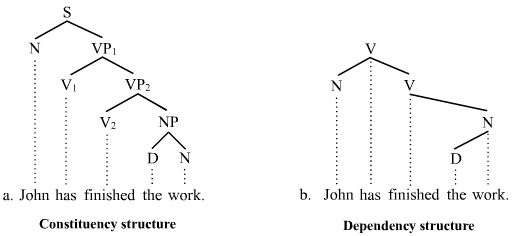
\includegraphics[width=0.7\textwidth]{figures/Johnhasfinishedthework}
	\caption{Parses of the sentence \textit{"John has finished the work"} \cite{parsers}}
	\label{fig:johnfinished}
\end{figure*}
%-------------------------------------------------------------
\section{Objectives}
The main focus of this study is computational semantics. Our research includes building explicit representations of natural language semantics, because in today's state-of-the art systems for popular semantics tasks such as measuring semantic similarity or machine comprehension, they are rarely present. Virtually all systems
competing at popular challenges (e.g. \cite{Cer:2017,Collados:2017}) rely on word embeddings as the sole representation of word meaning. Recently \cite{Recski:2016c} has presented a method using graphical representations of natural language text that improved over the state-of-the art on the task of
measuring semantic similarity of pairs of English words. In this paper
we use similar graphs as simple but powerful tools for measuring textual
entailment. Our task includes defining new methods for measuring graph similarities, and building an online available service for building graphs highly automatically, giving us a tool for building strong baseline methods. Our work was based upon measuring our models through state-of-the art systems on the 2018 Semeval Task \textit{Machine comprehension using commonsense knowledge}.

\section{Results}
We present a novel method for recognizing entailment using semantic
graphs and apply it to the 2018 Semeval task on Machine
Comprehension (MC).
Concept graphs are built automatically from MC texts, questions, and answers,
using the semantic parsing system \texttt{4lang} \cite{Recski:2016d}.
First we present a highly automated process of building concept graphs from raw text, then a strong baseline method is presented using only these graphs achieving an accuracy score of $68.3\%$,
followed by an enhancement of a state-of-the art system
\cite{Wang:2018}, where we proceeded to use the metric underlying our baseline as an additional feature. Preliminary results suggest that these features achieve a .5 percentage point improvement over the original system.

\section{References}
The code of our system is available on Github\footnote{\url{https://github.com/adaamko/4lang}}. The code was implemented by the authors of this paper based upon the \textbf{4lang} system.

\section{Structure}
The structure of the paper is the following:
\begin{itemize}
	\item \textbf{Chapter \ref{chap:Introdu}} describes the short history and motivation of the NLP applications, it also gives a short summary about the objectives of the paper, and our results.
	\item \textbf{Chapter \ref{chap:semanticparsing}} gives a short introduction into the field of semantic parsing, and semantic models in general. It briefly explains the semantic parsing system \textbf{4lang}, and our process of automating the building of concept graphs
	\item \textbf{Chapter \ref{chap:comprehension}} describes the baseline approach to the Machine Comprehension task, which achieved an accuracy score of $68.3\%$.
	\item \textbf{Chapter \ref{chap:deep}} gives an introduction into deep learning, focusing on the NLP tasks.
	\item \textbf{Chapter \ref{chap:yuanfudao}} presents our experiments with the state-of-the art system \textbf{Yuanfudao}. Our preliminary results show a .5 percent improvement over the original system.
	\item \textbf{Chapter \ref{chap:future}} summarizes our contributions and describes our ongoing/future work. It briefly discusses our plans for the follow-up, that was beyond the scope of this work.
\end{itemize}

\section{Division of labour}
This project was a product of the combined work of \vikszerzo and \vikszerzos. \vikszerzo was responsible for building the service to automate the process of building concept graphs (online demo available at \url{http://4lang.hlt.bme.hu}), and was mostly working on the baseline methods and metrics. \vikszerzos main work involved around applying the baseline to the state-of-the-art system Yuanfudao \cite{Wang:2018}.